% !TEX root = ../../main.tex

\chapter{Experiment Setup}

\label{chapter:experiment-setup}

\todo{Intro experimental environment}

\section{Software}

\todo{Detail software packages and such}
\todo{Answer RQ.1 by showing contribution C.1 "GPU optimized implementation of Amalur’s Factorized Machine Learning frame-
work"}


\section{Hardware}
\todo{Table showing different machines tested on}

\begin{table}[ht]
    \centering
    \begin{tabular}{@{}lll@{}}
    \toprule
    Experiment & Machine & Dataset type \\ \midrule \midrule
    CPU-1               & TUD st4          & train                 \\
    CPU-2               &                  & train                 \\
    CPU-3               &                  & train                 \\
    CPU-4               &                  & test                  \\ \midrule
    GPU-1               & TUD st4          & train                 \\
    GPU-2               &                  & train                 \\
    GPU-3               &                  & train                 \\
    GPU-4               &                  & test                  \\ \bottomrule
    \end{tabular}
    \caption{Overview of machines experiments will be run on.}
    \label{tab:my_label}
\end{table}

\section{Validation Strategy}
\todo{Explain how the collected metrics are divided into separate train \& test set to test generalizability}

\begin{figure}[ht]
    \centering
    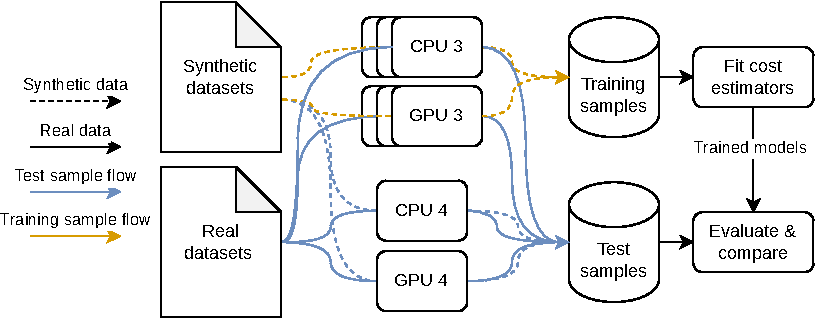
\includegraphics[width=0.8\linewidth]{chapters/05_experiment_setup/figures/experiment-pipeline.pdf}
    \caption{Overview of the planned experiments: combinations of datasets and machines we run the experiments
on. }
    \label{fig:enter-label}
\end{figure}

